\chapter{绪论}\label{cha:intro}
本章首先阐述论文的选题背景和意义(\ref{sec:background}节);随后介绍与工作流网相关的预备知识(\ref{sec:preliminaries}节);\ref{sec:challenge}节重点讨论基于工作流网的流程模型行为语义刻画方法当前所面临的挑战;\ref{sec:contribution}节给出论文的主要贡献;最后\ref{sec:structure}节介绍论文的章节安排。

\section{选题背景和意义}\label{sec:background}
如今信息系统需要支持业务流程的执行,而不是像以往一样仅仅关注于独立的任务。信息系统需要控制、监控并且支持一个业务流程逻辑层面的全部内容,即它应该能管理组织内的工作流。很多拥有大量业务流程的组织和企业对工作流的管理有着极为迫切的需求,这正是工作流管理兴起的原因\cite{van1998application}。在工作流管理技术的帮助下,企业可以快速建立或者更新自身的流程感知信息系统\cite{dumas2005process}。企业可以根据市场变化或者政府政策变更等外部因素随时调整自己的业务流程从而及时地改善自身的服务以提高企业的市场竞争力。

流程感知信息系统是由实际业务流程模型驱动的,这些模型描述了企业中的业务执行过程,每个任务的负责人以及需要的资源和产生的数据等。由于同一个业务流程可以被不同拓扑结构的图形所表示,因此它的行为语义才是刻画该流程的本质特征。任务间有序关系\cite{esparza2002improvement}常常被用来描述业务流程的行为。业务流程的任务间有三种基本的有序关系:因果关系(causal relation)描述一个任务的完成导致了另一个任务被执行,并行关系(concurrency relation)表示两个任务可以同时执行互不影响,冲突关系(conflict relation)表示在业务流程的同一个执行实例中两个任务不能都被执行。

两个有因果关系或者并行关系的任务可能在同一个流程执行实例中出现,但是在部分执行实例中一个任务被执行,另一个任务的执行却不是必然的。因此,本文对这两种有序关系进行精炼以体现这种不确定性。处于冲突关系的两个任务显然不能在同一个执行实例中出现,所以没有必要对冲突关系进行精炼。

\begin{figure}[htbp]
  \centering
  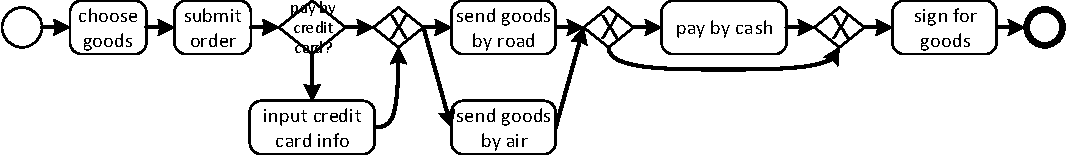
\includegraphics[width=1.0\textwidth]{basic_causal_drawback}
  \caption{含有不同因果关系的在线购物BPMN模型\label{fig:basic_causal_drawback}}
\end{figure}

\begin{example}\label{ex:basic_causal_drawback}
图\ref{fig:basic_causal_drawback}展示了一个在线购物的BPMN模型\footnote{BPMN是一种工作流建模语言,请参见:http://www.bpmn.org/}。在这个模型中,当任务“choose goods”被执行后,任务“submit order”可以被执行,然后任务“send goods by road”和任务“send goods by air”的其中之一可以被执行。显然,任务“choose goods”和任务“submit order”、任务“submit order”和任务“send goods by road”都满足因果关系。然而,这两组因果关系是不完全相同的。当任务“choose goods”被执行后,任务“submit order”一定会被执行而当任务“submit order”被执行后,任务“send goods by road”却不一定会被执行(因为任务“send goods by air”可能被选择执行)。前文提到的基本因果关系不能表达这类不同,所以需要对因果关系进行精炼。
\end{example}

\begin{figure}[htbp]
  \centering
  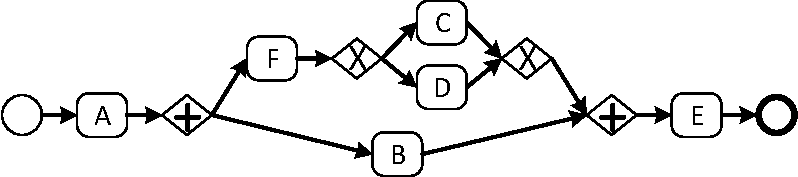
\includegraphics[width=0.8\textwidth]{basic_concurrency_drawback}
  \caption{含有不同并行关系的BPMN模型\label{fig:basic_concurrency_drawback}}
\end{figure}

\begin{example}\label{ex:basic_concurrency_drawback}
图\ref{fig:basic_concurrency_drawback}展示了一个含有并行结构的BPMN模型。在这个模型中,任务“B”和任务“C”可以被并行地执行但当任务“B”被执行时,任务“C”不一定会在同一个执行实例中被执行(因为任务“D”可能被选择执行)。同时,任务“B”和任务“F”也可以被并行地执行而且当任务“B”被执行时,任务“F”一定会在同一个执行实例中被执行。前文提到的基本并行关系不能表达这类不同,所以需要对并行关系进行精炼。
\end{example}

流程模型的任务间不确定性精炼有序关系(以下简称“精炼有序关系”)可以用来刻画流程的行为语义,从而被用于流程模型的检索,即提供一个查询模型$M$和一个流程模型集合$C$,从$C$中查找和$M$行为一致或者最相似的模型。由于本文的方法对流程模型进行了唯一的刻画,所以在检索过程中可以设置不同的粒度以检索符合实际要求的模型。除此之外,精炼有序关系还可以应用于流程模型的符合性检测、相似性度量等领域。

\begin{figure}[htbp]
  \centering
  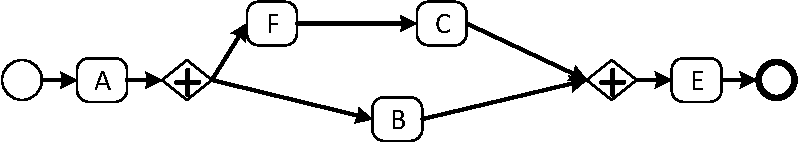
\includegraphics[width=0.8\textwidth]{basic_concurrency_drawback_compare}
  \caption{由图\ref{fig:basic_concurrency_drawback}改造得到的BPMN模型\label{fig:basic_concurrency_drawback_compare}}
\end{figure}

\begin{example}\label{ex:basic_concurrency_drawback_compare}
考虑图\ref{fig:basic_concurrency_drawback}和图\ref{fig:basic_concurrency_drawback_compare}中的模型,当检索满足条件“任务`F'和任务`C'满足因果关系且任务`B'和任务`C'满足并行关系”的模型时,两个模型都符合检索条件。另一方面,将检索条件更改为“任务`F'和任务`C'满足因果关系,且当任务`F'被执行时,任务`C'一定在同一个执行实例中被执行,同时当任务`C'被执行时,任务`F'一定在同一个执行实例中被执行;任务`B'和任务`C'满足并行关系,当任务`B'被执行时,任务`C'一定在同一个执行实例中被执行,同时当任务`C'被执行时,任务`B'一定在同一个执行实例中被执行”时,只有图\ref{fig:basic_concurrency_drawback_compare}中的模型符合条件。显然,精炼后的任务间有序关系能够更加精确地刻画流程模型的行为语义。类似的,这种精炼后的刻画方法可以被当作业务规则用于流程模型的符合性检测。
\end{example}

Jin等人已经提出了一种精炼有序关系RORU及其计算方法\cite{jin2014computing},本文重点对其进行了研究。针对该方法存在的问题,本文提出了改进方案,将新的方法命名为扩展的任务间不确定性精炼有序关系(Extended Refined Ordering Relations with Uncertainty,简称ExRORU)。由于ExRORU是一种刻画流程行为语义的方法,因此在实验过程中,本文将ExRORU与基于行为语义的流程特征刻画算法和流程相似性度量算法进行比较。

\section{预备知识}\label{sec:preliminaries}

\section{当前面临的挑战}\label{sec:challenge}

\section{论文的主要贡献}\label{sec:contribution}

\section{论文章节安排}\label{sec:structure}